% -*- mode: latex; -*- mustache tags:  
\documentclass[10pt,twoside,english]{_support/latex/sbabook/sbabook}
\let\wholebook=\relax

\usepackage{import}
\subimport{_support/latex/}{common.tex}

%=================================================================
% Debug packages for page layout and overfull lines
% Remove the showtrims document option before printing
\ifshowtrims
  \usepackage{showframe}
  \usepackage[color=magenta,width=5mm]{_support/latex/overcolored}
\fi


% =================================================================
\title{Documentation for Pharo Polyglot}
\author{Nikhil Pinnaparaju}
\series{Square Bracket tutorials}

\hypersetup{
  pdftitle = {Documentation for Pharo Polyglot},
  pdfauthor = {Nikhil Pinnaparaju},
  pdfkeywords = {NLP, Polyglot, Pharo, Smalltalk}
}


% =================================================================
\begin{document}

% Title page and colophon on verso
\maketitle
\pagestyle{titlingpage}
\thispagestyle{titlingpage} % \pagestyle does not work on the first one…

\cleartoverso
{\small

  Copyright 2017 by Nikhil Pinnaparaju.

  The contents of this book are protected under the Creative Commons
  Attribution-ShareAlike 3.0 Unported license.

  You are \textbf{free}:
  \begin{itemize}
  \item to \textbf{Share}: to copy, distribute and transmit the work,
  \item to \textbf{Remix}: to adapt the work,
  \end{itemize}

  Under the following conditions:
  \begin{description}
  \item[Attribution.] You must attribute the work in the manner specified by the
    author or licensor (but not in any way that suggests that they endorse you
    or your use of the work).
  \item[Share Alike.] If you alter, transform, or build upon this work, you may
    distribute the resulting work only under the same, similar or a compatible
    license.
  \end{description}

  For any reuse or distribution, you must make clear to others the
  license terms of this work. The best way to do this is with a link to
  this web page: \\
  \url{http://creativecommons.org/licenses/by-sa/3.0/}

  Any of the above conditions can be waived if you get permission from
  the copyright holder. Nothing in this license impairs or restricts the
  author's moral rights.

  \begin{center}
    
\includegraphics[width=0.2\textwidth]{_support/latex/sbabook/CreativeCommons-BY-SA.pdf}
  \end{center}

  Your fair dealing and other rights are in no way affected by the
  above. This is a human-readable summary of the Legal Code (the full
  license): \\
  \url{http://creativecommons.org/licenses/by-sa/3.0/legalcode}

  \vfill

  % Publication info would go here (publisher, ISBN, cover design…)
  Layout and typography based on the \textcode{sbabook} \LaTeX{} class by Damien
  Pollet.
}


\frontmatter
\pagestyle{plain}

\tableofcontents*
\clearpage\listoffigures

\mainmatter

\part{Documentation for Pharo Polyglot}
\chapter{DataFrame by example}
In this chapter, I will guide you through the complete functionality of the DataFrame project by showing examples of how each of those features can be used. This is a documentation of DataFrame written in a form of storytelling with data.
\section{Weather dataset}\label{weatherDataset}
For the demonstrational purposes, I have designed a simple dataset of meteorological observations. Imagine that to study the weather in certain area, you are collecting data by measuring the temperature and logging the type of precipitation (rain, snow etc.) every 20 minutes. The initial table contains only 5 observations (rows) and 3 features (columns): \textcode{temperature}, \textcode{precipitation}, and \textcode{type}. You can see this table in the top left of Figure \ref{weatherDataFrame}. As we progress through this chapter, we will be modifying, adding, and removing rows and columns of this dataset. Two additional columns that we will add are \textcode{humidity} and \textcode{wind}.


\begin{figure}

\begin{center}
\includegraphics[width=0.8\textwidth]{/home/cyber/Work/Pharo/Booklet-Polyglot/_result/pdf/Chapters/Chapter1/Images/weather.png}\caption{Weather data frame and two data series extracted from it: homogeneous series of temperature column and heterogeneous series of the third row\label{weatherDataFrame}}\end{center}
\end{figure}

\section{What are data frames and data series}
Before moving forward, you need to get a better understanding of the basic data structures that we use to model tabular data. In this section, I will explain the theoretical aspects of data frame and data series collections.

Data frame is a table of data. Similar to Excel spreadsheet or a relational database, but implemented as a collection that can be stored in a variable, such as \textcode{Array} or \textcode{Dictionary}. This greatly simplifies the data analysis workflow. Because, to answer questions such as \textit{\symbol{34}What was the temperature at 01:30?\symbol{34}} or \textit{\symbol{34}What is the average humidity when it snows?\symbol{34}}, we do not need to set up a whole database. Instead, we can simply load our data into a variable and query it - all in three lines of code (you will learn how to do it by reading the rest of this chapter):

\begin{displaycode}{plain}
weather := DataFrame readFromCsv: 'weather.csv'.

"Question 1"
weather at: 01:30 at: #temperature.

"Question 2"
(weather group: #temperature by: #type aggregateUsing: #average) at: #snow.
\end{displaycode}

In the top left of Figure \ref{weatherDataFrame}, you can see our weather dataset represented as a data frame. It contains three columns: \textcode{Float} column of temperatures, \textcode{Boolean} column which tells you whether or not there were any precipitations, and a \textcode{String} column that specifies the type of precipitation. Data types of columns are represented with different background colors.

It is common to think of rows as observations and columns as features. Therefore, columns are usually homogeneous - they contain values of a same data type, and rows can be heterogeneous - contain values of different types, such as \textcode{Integer}, \textcode{Float}, \textcode{Boolean}, \textcode{String}, etc.

Each row or column can be extracted as a \textcode{DataSeries} object - a dictionary of key-value pairs with a name. The keys of a row are the column nemes and for a column there are the row names of a data frame. This means that, by having those keys and a name, every individual row or column contains all the information that is needed to identify its precise location in a data frame, as well as the meaning of each value. As a result, data series is much more interpretable than a simple array of values, which allows us to construct more meaningful queries while analysing the dataset. We can add two series together, multiply them by a number, calculate the variance or standard deviation of a series, select elements that satisfy a certain condition, and do many other things that will be described in the following sections.

You can see the example of two data series in the top right and bottom of Figure \ref{weatherDataFrame}. Column \textcode{temperature} is a homogeneous \textcode{Float} data series and the row \textcode{01:50} is a heterogeneous series containing different types of values.

In the following section I will show you how to create a weather data frame and analyse it in Pharo. But first you need to install DataFrame v2.0 and make sure that all its tests are passing.
\section{Installation}
To install DataFrame, go to the Playground (Ctrl+O+W) in your fresh Pharo image and execute the following Metacello script (select it and press Do-it button or Ctrl+D):

\begin{displaycode}{smalltalk}
Metacello new
  baseline: 'DataFrame';
  repository: 'github://PolyMathOrg/DataFrame/src';
  load.
\end{displaycode}

In all keyboard shortcuts mentioned in this booklet the \textit{Ctrl} key is for Windows and Linux. On Mac OS, use \textit{Cmd} instead.
\subsection{Running the tests}
First thing you should do after installing DataFrame is open the DataFrame-Tests package in Test Runner (Ctrl+O+U) or System Browser (Ctrl+O+B) and make sure that all tests are passing. DataFrame v2.0 is tested with 301 unit tests which provide 90\% code coverage. If you see some failing tests, please go to the DataFrame repository on GitHub and open a related issue.
\section{Creating a data series}\label{secCreatingDataSeries}
\textcode{DataSeries} behaves like an \textcode{OrderedDictionary}. You can create it by providing keys, values, and a name:

\begin{displaycode}{plain}
DataSeries
  withKeys: (#('01:10' '01:30' '01:50' '02:10' '02:30') collect: #asTime)
  values: #(2.4 0.5 -1.2 -2.3 3.2)
  name: #temperature.
\end{displaycode}

This creates the first column of our weather data frame.

\begin{tabular}{ll}
\toprule
 & \textbf{temperature} \\
\midrule
\textbf{1:10 am} & 2.4 \\
\textbf{1:30 am} & 0.5 \\
\textbf{1:50 am} & -1.2 \\
\textbf{2:10 am} & -2.3 \\
\textbf{2:30 am} & 3.2 \\
\bottomrule
\end{tabular}

If you don't specify a name, it will be set to the default value \textcode{'(no name)'}:

\begin{displaycode}{plain}
DataSeries
  withKeys: #(temperature precipitation type)
  values: #(0.5 true rain).
\end{displaycode}

\begin{tabular}{ll}
\toprule
 & \textbf{(no name)} \\
\midrule
\textbf{temperature} & 0.5 \\
\textbf{precipitation} & true \\
\textbf{type} & rain \\
\bottomrule
\end{tabular}

You can also create a data series without keys, in which case they fill be filled with default values: numbers from 1 to the size of your data series:

\begin{displaycode}{plain}
temperature := DataSeries
  withValues: #(2.4 0.5 -1.2 -2.3 3.2)
  name: #temperature.
\end{displaycode}

\begin{tabular}{ll}
\toprule
 & \textbf{temperature} \\
\midrule
\textbf{1} & 2.4 \\
\textbf{2} & 0.5 \\
\textbf{3} & -1.2 \\
\textbf{4} & -2.3 \\
\textbf{5} & 3.2 \\
\bottomrule
\end{tabular}

Or only with values:

\begin{displaycode}{plain}
DataSeries
  withValues: #(2.4 0.5 -1.2 -2.3 3.2).
\end{displaycode}

\begin{tabular}{ll}
\toprule
 & \textbf{(no name)} \\
\midrule
\textbf{1} & 2.4 \\
\textbf{2} & 0.5 \\
\textbf{3} & -1.2 \\
\textbf{4} & -2.3 \\
\textbf{5} & 3.2 \\
\bottomrule
\end{tabular}

That last expression has a shorter form which produces the same result:

\begin{displaycode}{plain}
#(2.4 0.5 -1.2 -2.3 3.2) asDataSeries.
\end{displaycode}
\section{Discovering data series API}
\textcode{DataSeries} is an extended \textcode{OrderedDictionary}. It combines the API of both \textcode{Dictionary} and \textcode{SequenceableCollection}, and adds some additional functionality that can be useful for data analysis. This simple data structure does not require a long introduction but it is still worth to demonstrate how it can be used. In this section, I briefly cover the public API of a \textcode{DataSeries} class and describe the additional methods that are not present in other Pharo collections.
\subsection{Accessing and modifying values}
In this aspect, \textcode{DataSeries} acts like an \textcode{OrderedDictionary}. You can access an element at a certain key using \textcode{at: aKey} message, you can modify this element with \textcode{at: aKey put: newValue}. To remove an element, use \textcode{removeAt: aKey}. If \textcode{aKey} is not present in the data series, a new element will be created and added to the end. Alternatively, you can use methods such as \textcode{at: ifAbsent:}, \textcode{at: ifAbsentPut:}, etc. to provide custom block that will be evaluated when \textcode{aKey} is not found.

You can also access elements by their index rather than key with methods \textcode{atIndex:}, \textcode{atIndex: put:}, and \textcode{removeAtIndex:}.

Here is the list of some accessors provided by \textcode{DataSeries}. This list is incomplete. Many other accessors are inherited from \textcode{OrderedCollection} class. They can come in handy but we do not discuss them in this booklet:

\begin{displaycode}{plain}
DataSeries >> at:
DataSeries >> at: ifAbsent:
DataSeries >> at: put:
DataSeries >> removeAt:
DataSeries >> atIndex:
DataSeries >> atIndex: put:
DataSeries >> removeAtIndex:
\end{displaycode}

Now we present the non traditional and powerful API of \textcode{DataSeries}.
\section{at:transform:}\label{secAtTransform}
\textcode{DataSeries} provides additional set of \textcode{at: transform:} modifying accessors. Consider a situation when you want to convert a certain value of the temperature data series from Celsius to Fahrenheit. Having to specify key twice we make the whole expression long and hard to comprehend:

\begin{displaycode}{plain}
temperature at: '01:30' asTime put: (temperature at: '01:30' asTime)  * 9/5 + 32.
\end{displaycode}

And since operations on data series (rows and columns) are the building block of most data frame queries, we want them to be as short and readable as possible. To simplify complex queries, \textcode{DataSeries} provides a set of methods that allow you to transform an element at certain position using a block:

\begin{displaycode}{plain}
DataSeries >> at: transform:
DataSeries >> at: transform: ifAbsent:
DataSeries >> atIndex: transform:
\end{displaycode}

We can now rewrite the above expression as

\begin{displaycode}{plain}
temperature at: '01:30' asTime transform: [ :x | x * 9/5 + 32 ].
\end{displaycode}
\section{Enumerating values of data series}\label{secEnumeratingSeries}
As a combination of \textcode{Dictionary} and \textcode{SequenceableCollection}, \textcode{DataSeries} understands the following methods for enumerating its values:

\begin{tabular}{lll}
\toprule
\textbf{Value} & \textbf{Value and key} & \textbf{Value and index} \\
\midrule
do: & withKeyDo: & withIndexDo: \\
select: & withKeySelect: & withIndexSelect: \\
reject: & withKeyReject: & withIndexReject: \\
collect: & withKeyCollect: & withIndexCollect: \\
detect: & withKeyDetect: & withIndexDetect: \\
detect: ifNone: & withKeyDetect: ifNone: & withIndexDetect: ifNone: \\
inject: into: & - & - \\
\bottomrule
\end{tabular}

For example, we can collect the Fahrenheit values of \textcode{temperature} into a separate series:

\begin{displaycode}{plain}
fahrenheit := temperature collect: [ :x | x * 9/5 + 32 ].
\end{displaycode}

\begin{tabular}{ll}
\toprule
 & \textbf{temperature} \\
\midrule
\textbf{1} & 36.32 \\
\textbf{2} & 32.9 \\
\textbf{3} & 29.84 \\
\textbf{4} & 27.86 \\
\textbf{5} & 37.76 \\
\bottomrule
\end{tabular}

Notice that the name of this data series is still \textcode{temperature}, because that was the name of a series from which the values were collected, and no other name was provided by the \textcode{collect:} message. If needed, you can rename the \textcode{fahrenheit} series later:

\begin{displaycode}{plain}
fahrenheit name: #fahrenheit.
\end{displaycode}

To see another example of enumerating values of data series, let's now find the first value of the \textcode{fahrenheit} series that is below 32 (zero on Celsius scale):

\begin{displaycode}{plain}
fahrenheit detect: [ :x | x < 32 ].
\end{displaycode}

The answer will be \textcode{29.84} - the third element of our series.
\section{Arithmetical operations}
Similarly to other collections in Pharo, \textcode{DataSeries} responds to basic arithmetical operations, such as \textcode{+, -, *, /}. You can apply these operations on any of the following combinations: series-series, series-scalar, or scalar-series (although, the last one is not supported for division).

In order to demonstrate the application of arithmetical operations, let's create two simple data series filled with numbers:

\begin{displaycode}{plain}
a := DataSeries withValues: #(0.5 2 -1 0) name: #a.
b := DataSeries withValues: #(-2 -0.5 1 3) name: #b.
\end{displaycode}

When an operation is applied to a scalar and a series, it is performed on every element of a series with the given scalar. For example, if you divid data series \textcode{a} by 2, each of its elements will be divided by 2:

\begin{displaycode}{plain}
a / 2.
\end{displaycode}

\begin{tabular}{ll}
\toprule
 & \textbf{a} \\
\midrule
\textbf{1} & 0.25 \\
\textbf{2} & 1 \\
\textbf{3} & -0.5 \\
\textbf{4} & 0 \\
\bottomrule
\end{tabular}

Similarly, if you subtract data series \textcode{b} from the number 1, you will get a new series, in which each element is the difference between 1 and the corresponding element of series \textcode{b}:

\begin{displaycode}{plain}
1 - b.
\end{displaycode}

\begin{tabular}{ll}
\toprule
 & \textbf{b} \\
\midrule
\textbf{1} & 3 \\
\textbf{2} & 1.5 \\
\textbf{3} & 0 \\
\textbf{4} & -2 \\
\bottomrule
\end{tabular}

When the operation is applied to a pair of two data series, it will be performed in the elementwise manner. So, for example, if you want to add two data series \textcode{a} and \textcode{b}, you will get a third series where first element is the sum of the first elements of \textcode{a} and \textcode{b}, second element is the sum of second elements, etc. In this case, both data series must be of the same size and must have same keys. The name of the resulting series will be the same as the name of the first operand:

\begin{displaycode}{plain}
a + b.
\end{displaycode}

\begin{tabular}{ll}
\toprule
 & \textbf{a} \\
\midrule
\textbf{1} & -1.5 \\
\textbf{2} & 1.5 \\
\textbf{3} & 0 \\
\textbf{4} & 3 \\
\bottomrule
\end{tabular}

In fact, the conversion of \textcode{temperature} series to Fahrenheit scale, that was demonstrated earlier in Section \ref{secEnumeratingSeries} with \textcode{collect:} message, can be done directly by applying arithmetical operations to the data series:

\begin{displaycode}{plain}
fahrenheit := temperature * 9/5 + 32.
\end{displaycode}

The result will be the same as before.
\section{Some useful mathematical functions}
Although, you can apply any operation to the elements of your series using \textcode{collect:}, sometimes your code will be more readable if you send a message to the whole data series and expect it to be performed on all its elements. In the same way as when we add 1 to a data series and get a new series with all elements of the first series incremented by 1, we also want to say \textcode{series exp} and expect a data series of exponents.

Here is the list of mathematical operations that are understood by \textcode{DataSeries} and can be performed in the elementwise manner:

\begin{displaycode}{plain}
DataSeries >> abs
DataSeries >> cos
DataSeries >> sin
DataSeries >> tan
DataSeries >> exp
DataSeries >> ln
DataSeries >> log
DataSeries >> log:
DataSeries >> sqrt
DataSeries >> **
\end{displaycode}

The last one is the binary operator which takes data series as the first operand and raises all its elements to the power of second operand.

Let's find the exponent and the natural logarithm of the temperature series:

\begin{displaycode}{plain}
temperature exp.
\end{displaycode}

\begin{tabular}{ll}
\toprule
 & \textbf{temperature} \\
\midrule
\textbf{1} & 11.02 \\
\textbf{2} & 1.65 \\
\textbf{3} & 0.3 \\
\textbf{4} & 0.1 \\
\textbf{5} & 24.53 \\
\bottomrule
\end{tabular}

As we take the natural logarithm, the third and fourth elements in the resulting data series are \textcode{Float nan} because logarithms are only defined for positive numbers and those two temperatures are below zero:

\begin{displaycode}{plain}
temperature ln.
\end{displaycode}

\begin{tabular}{ll}
\toprule
 & \textbf{temperature} \\
\midrule
\textbf{1} & 0.88 \\
\textbf{2} & -0.69 \\
\textbf{3} & Float nan \\
\textbf{4} & Float nan \\
\textbf{5} & 1.16 \\
\bottomrule
\end{tabular}

\begin{note}
Unlike most other programming languages and libraries for numerical coomputations that define \textcode{log} as natural logarithm, Pharo defines it as a logarithm with base 10. Natural logarithm is defined as \textcode{ln}. And parametrised message \textcode{log:} can be used to get a logarithm with any other base, for example: \textcode{(1024 log: 2) = 10.0}.
\end{note}
\section{Statistical operations}
In addition to statistical methods understood by all collections, such as \textcode{average}, \textcode{min}, or \textcode{max}, \textcode{DataSeries} class provides methods more advanced methods that are commonly used when analysing quantitative columns. Here is the complete list of statistical methods understood by \textcode{DataSeries}:

\begin{displaycode}{plain}
DataSeries >> min
DataSeries >> max
DataSeries >> range
DataSeries >> average
DataSeries >> median
DataSeries >> mode
DataSeries >> quantile:
DataSeries >> quartile:
DataSeries >> zerothQuartile
DataSeries >> firstQuartile
DataSeries >> secondQuartile
DataSeries >> thirdQuartile
DataSeries >> fourthQuartile
DataSeries >> interquartileRange
\end{displaycode}

If any of these methods is applied to a non-numerical data series, it will signal an exception.

To demonstrate the application of statistical methods, let's find average, median, standard deviation, and variance of the temperature column:

\begin{displaycode}{plain}
temperature average. "0.52"
temperature median. "0.5"
temperature stdev. "2.3253"
temperature variance. "5.407"
\end{displaycode}

We can also check if the following equalities hold: zeroth quartile should be the same as min, fourth quartile should be the same as max, second quartile - same as median, interquartile range equals third quartile minus the first one, range is max minus min, and variance is the square of standard deviation:

\begin{displaycode}{plain}
temperature zerothQuartile = temperature min. "true"
temperature fourthQuartile = temperature max. "true"
temperature secondQuartile = temperature median. "true"
temperature interquartileRange = (temperature thirdQuartile - temperature firstQuartile). "true"
temperature range = (temperature max - temperature min). "true"
temperature variance = (temperature stdev ** 2). "true"
\end{displaycode}
\subsection{Summarizing a DataSeries}
You can get a quick summary of the distribution of a numerical data series as a collection of its minimal and maximal values, first and third quartiles, average value, and a median.

Let's see how it works for the temperature series created in \ref{secCreatingDataSeries}:

\begin{displaycode}{plain}
temperature summary.
\end{displaycode}

\begin{tabular}{ll}
\toprule
 & \textbf{temperature} \\
\midrule
\textbf{Min} & -2.3 \\
\textbf{1st Qu.} & -1.2 \\
\textbf{Median} & 0.5 \\
\textbf{Average} & 0.52 \\
\textbf{3rd Qu.} & 2.4 \\
\textbf{Max} & 3.2 \\
\bottomrule
\end{tabular}
\section{Working with categorical values}
Categorical data series have a fixed dictionary of values. For example, series \textcode{sex} which has values \textcode{Male} and \textcode{Female}, boolean series with values \textcode{true} and \textcode{false}, series with sizes of clothes: \textcode{XS}, \textcode{S}, \textcode{M}, \textcode{L}, \textcode{XL}, etc. We can not perform mathematical and statistical operations on categorical series (except for \textcode{mode}, which only finds the most common value), however there is still a lot of ways to analyse such data. In the rest of this section, I will show you several methods of \textcode{DataSeries} that are especially useful for working with categorical values. The examples will be based on the \textcode{precipitation} and \textcode{type} columns of weather dataset. I remind you how they are created:

\begin{displaycode}{plain}
keys := #('01:10' '01:30' '01:50' '02:10' '02:30') collect: #asTime.

precipitation := DataSeries
  withKeys: keys
  values: #(true true true false true)
  name: #precipitation.

type := DataSeries
  withKeys: keys
  values: #(rain rain snow - rain)
  name: #type.
\end{displaycode}
\subsection{uniqueValues}
The most basic operation that can be performed is finding the unique values of the series:

\begin{displaycode}{plain}
precipitation uniqueValues. "#(false true)"
type uniqueValues. "#(- rain snow)"
\end{displaycode}

This allows us to see the complete dictionary of values used in a data series.
\subsection{valueCounts}
Another thing you might want to know is how the values of your categorical data series are distributed. How many times did it rain, according to your dataset? How many times did it snow? \textcode{valueCounts} method will give you the counts of unique values in your data series:

\begin{displaycode}{plain}
type valueCounts.
\end{displaycode}

\begin{tabular}{ll}
\toprule
 & \textbf{type} \\
\midrule
\textbf{rain} & 3 \\
\textbf{snow} & 1 \\
\textbf{-} & 1 \\
\bottomrule
\end{tabular}

The result will be a data series with unique values as keys and counts as values. It will be sorted by counts in the descending order.
\subsection{valueFrequencies}
Sometimes, instead of counts, you want to see the relative frequencies of the unique values in your data series:

\begin{displaycode}{plain}
type valueFrequencies.
\end{displaycode}

\begin{tabular}{ll}
\toprule
 & \textbf{type} \\
\midrule
\textbf{rain} & (3/5) \\
\textbf{snow} & (1/5) \\
\textbf{-} & (1/5) \\
\bottomrule
\end{tabular}

In fact, it is the same as dividing value counts by the size of your series:

\begin{displaycode}{plain}
type valueFrequencies = (type valueCounts / type size). "true"
\end{displaycode}
\subsection{crossTabulateWith:}
Cross tabulation is a powerful way to analyse the correlation between two categorical series. It creates a table with rows corresponding to the unique values of the first series, columns corresponding to the unique values of second series, and each cell containing the count of those value pairs.

By cross tabulating \textcode{precipitation} series with \textcode{type} series, we can see that they are closely correlated - when \textcode{precipitation} is \textcode{false}, the \textcode{type} is always empty, and when \textcode{precipitation} is \textcode{true}, the \textcode{type} is either \textcode{rain} or \textcode{snow}:

\begin{displaycode}{plain}
precipitation crossTabulateWith: type.
\end{displaycode}

The result will be the data frame of cross tabulated values:

\begin{tabular}{llll}
\toprule
 & \textbf{snow} & \textbf{rain} & \textbf{-} \\
\midrule
\textbf{false} & 0 & 0 & 1 \\
\textbf{true} & 1 & 3 & 0 \\
\bottomrule
\end{tabular}
\section{Creating a data frame}
In this section, we will look at different ways of creating the weather data frame described in Section \ref{weatherDataset}.
You will also learn to create empty data frames that can be filled with values later.
\subsection{Initializing a data frame with an array of rows}
The most basic way to initialize a data frame is with an array (or any other ordered collection) of rows where each row is a collection of elements. Let's create the weather data frame from its rows:

\begin{displaycode}{plain}
weather := DataFrame withRows: #(
	(2.4 true rain)
	(0.5 true rain)
	(-1.2 true snow)
	(-2.3 false -)
	(3.2 true rain)).
\end{displaycode}
\subsection{Initializing a data frame with an array of columns}
Alternatively, you can create a data frame by passing it a collection of columns. This can be handy, for example, when engineering new features: \textcode{DataFrame withColumns: \{ income . income ** 2 . income log \}}. In our case, we create the same weather data frame:

\begin{displaycode}{plain}
weather := DataFrame withColumns: #(
  (2.4 0.5 -1.2 -2.3 3.2)
  (true true true false true)
  (rain rain snow - rain)).
\end{displaycode}
\subsection{Specifying column and row names}
Both expressions in two previous sections create the same data frame.

\begin{tabular}{llll}
\toprule
 & \textbf{1} & \textbf{2} & \textbf{3} \\
\midrule
\textbf{1} & 2.4 & true & rain \\
\textbf{2} & 0.5 & true & rain \\
\textbf{3} & -1.2 & true & snow \\
\textbf{4} & -2.3 & false & - \\
\textbf{5} & 3.2 & true & rain \\
\bottomrule
\end{tabular}

Since the names of rows and columns were not specified, they were initialized with their default values: \textcode{(1 to: self numberOfRows)} and \textcode{(1 to: self numberOfColumns)}. We can provide more meaningful names:

\begin{displaycode}{plain}
weather := DataFrame withColumns: #(
  (2.4 0.5 -1.2 -2.3 3.2)
  (true true true false true)
  (rain rain snow - rain)).

weather columnNames: #(temperature precipitation type).
weather rowNames: (#('01:10' '01:30' '01:50' '02:10' '02:30')
		collect: #asTime).
\end{displaycode}

I would like to emphasize that names don't have to be strings or numbers. They can be any objects, and in this case they are instances of Time. Now the data frame looks the same as the table in Figure \ref{weatherDataFrame} (A).

\begin{tabular}{llll}
\toprule
 & \textbf{temperature} & \textbf{precipitation} & \textbf{type} \\
\midrule
\textbf{1:10 am} & 2.4 & true & rain \\
\textbf{1:30 am} & 0.5 & true & rain \\
\textbf{1:50 am} & -1.2 & true & snow \\
\textbf{2:10 am} & -2.3 & false & - \\
\textbf{2:30 am} & 3.2 & true & rain \\
\bottomrule
\end{tabular}
\subsection{Compact methods for initializing data frames}
\textcode{DataFrame} class provides syntactic sugar that allows us to initialize it with contents and (optionally) row and column names in a single line. Here is the complete list of those initializers:

\begin{displaycode}{plain}
DataFrame class >> withRows: columnNames:
DataFrame class >> withRows: rowNames:
DataFrame class >> withRows: rowNames: columnNames:
DataFrame class >> withColumns: columnNames:
DataFrame class >> withColumns: rowNames:
DataFrame class >> withColumns: rowNames: columnNames:
\end{displaycode}

Whenever row or column names are not specified, they are initialized with their default values.
\section{Creating empty data frames}
Sometimes we need to create an empty data frame that will be filled with data later on. The easiest way of doing this is with

\begin{displaycode}{plain}
DataFrame new. "empty data frame with 0 rows and 0 columns"
\end{displaycode}

This will create an empty data frame with no columns and rows. You can also create an empty data frame of a given size by specifying it as a point \textcode{numberOfRows @ numberOfColumns}. All cells of such data frame will be empty (initialized with \textcode{nil}).

\begin{displaycode}{plain}
DataFrame new: 3@4. "empty data frame with 3 rows and 4 columns"
\end{displaycode}

Similarly to the syntactic sugar described in the previous section, DataFrame class has methods that allow us to create data frames by specifying only their rows, columns, or both. Since we do not provide any data, such data frames with be empty and their sizes will correspond to the provided arrays of rows and columns. For example, if you create an empty data frame with columns \textcode{\#(temperature precipitation type)}, its size will be \textcode{0@3}. Here are the methods that can be used to create an empty data frame with names:

\begin{displaycode}{plain}
DataFrame class >> withRowNames:
DataFrame class >> withColumnNames:
DataFrame class >> withRowNames: columnNames:
\end{displaycode}

For example, we can initialize an empty weather data frame:

\begin{displaycode}{plain}
emptyWeather := DataFrame
  withRowNames: (#('01:10' '01:30' '01:50' '02:10' '02:30') collect: #asTime)
  columnNames: #(temperature precipitation type).
\end{displaycode}

\begin{tabular}{llll}
\toprule
 & \textbf{temperature} & \textbf{precipitation} & \textbf{type} \\
\midrule
\textbf{1:10 am} & nil & nil & nil \\
\textbf{1:30 am} & nil & nil & nil \\
\textbf{1:50 am} & nil & nil & nil \\
\textbf{2:10 am} & nil & nil & nil \\
\textbf{2:30 am} & nil & nil & nil \\
\bottomrule
\end{tabular}

\begin{note}
Although it is possible to create a data frame with no rows using \textcode{DataFrame class \textgreater{}\textgreater{} new} or \textcode{DataFrame \textgreater{}\textgreater{} withColumnNames:} and add rows later by pushing them one by one, this is not recommended. DataFrame is not optimized for the insertion of new elements. It may be more efficient to first add rows into an OrderedCollection and then initialize a data frame with it.
\end{note}
\section{Inspecting a data frame}
It is hard to work with data tables without being able to see them. Fortunately, Pharo environment provides a powerful inspector which allows you examine live objects and even modify them. If you inspect a data frame object (select it anywhere in the code and press Ctrl+I or Ctrl+G if you are in Playground), you will see the table similar to the one in Figure \ref{inspector}.


\begin{figure}

\begin{center}
\includegraphics[width=1.0\textwidth]{/home/cyber/Work/Pharo/Booklet-Polyglot/_result/pdf/Chapters/Chapter1/Images/fastTableWhite.png}\caption{Inspecting weather data frame \label{inspector}}\end{center}
\end{figure}

\section{Accessing parameters of data frame}
Data frames are defined by their contents (table of data), as well as their column and row names. For the simplicity, we provide access to some additional parameters such as the dimensions of a data frame. In the following sections, we will discuss how to access row and columns, as well as its individual cells. In this section, I will show you how to get other parameters such as names or sizes.
\subsection{Dimensions}
Getting the number of rows and columns of a data frame is straightforward:

\begin{displaycode}{plain}
weather numberOfRows. "5"
weather numberOfColumns. "3"
\end{displaycode}

You can also get both dimensions of a data frame as a \textcode{Point}:

\begin{displaycode}{plain}
weather dimensions. "5@3"
\end{displaycode}
\subsection{Row and column names}
Every data frame has names associated to its rows and columns (either used-defined or auto-generated). These names can be used for referencing specific rows or columns (which you will learn in Section \ref{secAccessingByName}). Let's get the collection of all row and column names of a weather data frame:

\begin{displaycode}{plain}
weather rowNames.
weather columnNames.
\end{displaycode}
\subsection{Transposed DataFrame}
Sometimes it is useful to transpose a data frame made out of columns and rows into rows and columns. To do that, you can simply write

\begin{displaycode}{plain}
weather transposed
\end{displaycode}

The result will be a new data frame which looks like this:

\begin{tabular}{llllll}
\toprule
 & \textbf{1:10 am} & \textbf{1:30 am} & \textbf{1:50 am} & \textbf{2:10 am} & \textbf{2:30 am} \\
\midrule
\textbf{temperature} & 2.4 & 0.5 & -1.2 & -2.3 & 3.2 \\
\textbf{precipitation} & true & true & true & false & true \\
\textbf{type} & rain & rain & snow & - & rain \\
\bottomrule
\end{tabular}
\section{Accessing rows and columns}
In this section, I will show you how to get the values of specific rows and columns, as well as how to modify these values. Rows and columns of a data frame can be accessed either by their names or their numeric indexes.
\subsection{Accessing by name}\label{secAccessingByName}
You can get row \textcode{01:50} and the column \textcode{temperature} of the weather data frame by writing:

\begin{displaycode}{plain}
weather row: '01:50' asTime.
weather column: #temperature.
\end{displaycode}

Use methods \textcode{row: put:} and \textcode{column: put:} to modify the values stored in a row or column:

\begin{displaycode}{plain}
weather row: '01:50' asTime put: #(10 true rain).
weather column: #temperature put: #(1.2 -2.1 3.4 -5.9 -0.4).
\end{displaycode}

\begin{tabular}{llll}
\toprule
 & \textbf{temperature} & \textbf{precipitation} & \textbf{type} \\
\midrule
\textbf{1:10 am} & 1.2 & true & rain \\
\textbf{1:30 am} & -2.1 & true & rain \\
\textbf{1:50 am} & 3.4 & true & rain \\
\textbf{2:10 am} & -5.9 & false & - \\
\textbf{2:30 am} & -0.4 & true & rain \\
\bottomrule
\end{tabular}

If you reference a row or column by a non-existing name you will get the \textcode{NotFoundError} and if the array you provide is too big or too small, the \textcode{SizeMismatch} error will be signaled. Notice that you can not add a new column using \textcode{dataFrame column: \#newName put newArray}. This is done with \textcode{addColumn:} set of methods that will be described in the following sections.
\subsection{Accessing by index}
Rows and columns can also be accessed by their numeric indices. You can get the same row and column as in the previous example using

\begin{displaycode}{plain}
weather rowAt: 3.
weather columnAt: 1.
\end{displaycode}

To modify them, use \textcode{rowAt: put:} and \textcode{columnAt: put:}.

\begin{displaycode}{plain}
weather rowAt: 3 put: #(-1.2 true snow).
weather columnAt: 1 put: #(2.4 0.5 -1.2 -2.3 3.2).
\end{displaycode}

\begin{tabular}{llll}
\toprule
 & \textbf{temperature} & \textbf{precipitation} & \textbf{type} \\
\midrule
\textbf{1:10 am} & 2.4 & true & rain \\
\textbf{1:30 am} & 0.5 & true & rain \\
\textbf{1:50 am} & -1.2 & true & snow \\
\textbf{2:10 am} & -2.3 & false & - \\
\textbf{2:30 am} & 3.2 & true & rain \\
\bottomrule
\end{tabular}
\subsection{Accessing multiple rows and columns}
To access multiple rows or columns at a same time, you have to provide an array of names or indices, or specify the range of indices. In the following example, we get the three middle rows of the weather data frame:

\begin{displaycode}{plain}
weather rows: { '01:30' asTime . '01:50' asTime . '02:10' asTime}.
weather rowsAt: #(2 3 4).
weather rowsFrom: 2 to: 4.
\end{displaycode}

The same can be done to access, for example, the last two columns:

\begin{displaycode}{plain}
weather columns: #(precipitation type).
weather columnsAt: #(2 3).
weather columnsFrom: 2 to: 3.
\end{displaycode}

The result will be another data frame with only the requested rows or columns in the order in which you ask for them. This means that you can ask for rows 3, 2, and the 5 or column \textcode{precipitation} followed by the \textcode{temperature}:

\begin{displaycode}{plain}
weather rowsAt: #(3 2 5).
weather columns: #(precipitation temperature).
\end{displaycode}

All the above methods can be used together with \textcode{put:} to replace the given rows or columns with new ones:

\begin{displaycode}{plain}
DataFrame >> rows: put:
DataFrame >> rowsAt: put:
DataFrame >> rowsFrom: to: put:
DataFrame >> columns: put:
DataFrame >> columnsAt: put:
DataFrame >> columnsFrom: to: put:
\end{displaycode}
\subsection{Head and Tail}
To understand the nature of a dataset with 100,000 rows, it helps if we can take a look at its first or last 5 rows. This is called the \textbf{head} or \textbf{tail} of a dataset. \textcode{DataFrame} allows you to get the arbitrary number of rows at its beginning or end using \textcode{head: aNumber} and \textcode{tail: aNumber} methods. It also provides simpler methods \textcode{head} and \textcode{tail} which return 5 rows by default.

For example, if we want to get the first 2 rows from our weather data frame:

\begin{displaycode}{plain}
weather head: 2.
\end{displaycode}

\begin{tabular}{llll}
\toprule
 & \textbf{temperature} & \textbf{precipitation} & \textbf{type} \\
\midrule
\textbf{1:10 am} & 2.4 & true & rain \\
\textbf{1:30 am} & 0.5 & true & rain \\
\bottomrule
\end{tabular}

Or the tail with the last 3 rows:

\begin{displaycode}{plain}
weather tail: 2.
\end{displaycode}

\begin{tabular}{llll}
\toprule
 & \textbf{temperature} & \textbf{precipitation} & \textbf{type} \\
\midrule
\textbf{1:50 am} & -1.2 & true & snow \\
\textbf{2:10 am} & -2.3 & false & - \\
\textbf{2:30 am} & 3.2 & true & rain \\
\bottomrule
\end{tabular}

Both \textcode{head} and \textcode{tail} are returned to you as new data frames with only the corresponding rows. DataSeries also implements the \textcode{head}/\textcode{tail} methods, which allows you to get the \textcode{head} or \textcode{tail} of a single row or column as a new data series with only the first or last elements

\begin{displaycode}{plain}
(weather column: #temperature) head: 2.
\end{displaycode}

\begin{tabular}{ll}
\toprule
 & \textbf{temperature} \\
\midrule
\textbf{1:10 am} & 2.4 \\
\textbf{1:30 am} & 0.5 \\
\bottomrule
\end{tabular}
\section{Adding rows and columns}\label{secAddingRowsAndColumns}
You can add new rows and columns to data frame by providing an array of values a name of the new row or column, and its position as an index:

\begin{displaycode}{plain}
weather
  addColumn: #(86 79 23 16 90)
  named: #humidity
  atPosition: 2.
\end{displaycode}

The above statement will modify the weather dataset by adding a humidity column to it right after the temperature column:

\begin{tabular}{lllll}
\toprule
 & \textbf{temperature} & \textbf{humidity} & \textbf{precipitation} & \textbf{type} \\
\midrule
\textbf{1:10 am} & 2.4 & 86 & true & rain \\
\textbf{1:30 am} & 0.5 & 79 & true & rain \\
\textbf{1:50 am} & -1.2 & 23 & true & snow \\
\textbf{2:10 am} & -2.3 & 16 & false & - \\
\textbf{2:30 am} & 3.2 & 90 & true & rain \\
\bottomrule
\end{tabular}

You can omit the position using methods \textcode{addRow:named:} or \textcode{addColumn:named:}. By default rows and columns will be added to the end of data frame:

\begin{displaycode}{plain}
weather
  addRow: #(2.0 81 true rain)
  named: '2:50' asTime.
\end{displaycode}

\begin{tabular}{lllll}
\toprule
 & \textbf{temperature} & \textbf{humidity} & \textbf{precipitation} & \textbf{type} \\
\midrule
\textbf{1:10 am} & 2.4 & 86 & true & rain \\
\textbf{1:30 am} & 0.5 & 79 & true & rain \\
\textbf{1:50 am} & -1.2 & 23 & true & snow \\
\textbf{2:10 am} & -2.3 & 16 & false & - \\
\textbf{2:30 am} & 3.2 & 90 & true & rain \\
\textbf{2:50 am} & 2.0 & 81 & true & rain \\
\bottomrule
\end{tabular}

Alternatively, you can add new rows or columns as data series. In this case you do not need to provide a name because the data series already knows its name.

\begin{displaycode}{plain}
wind := DataSeries
  withValues: #(39 39 32 24 14 14)
  name: #wind.

weather
  addColumn: wind
  atPosition: 2.
\end{displaycode}

Notice that we did not specify the keys of the data series with wind measurements. It was initialized with default keys. When adding new row or column as a data series, \textcode{DataFrame} does not take keys into account.

\begin{tabular}{llllll}
\toprule
 & \textbf{temperature} & \textbf{wind} & \textbf{humidity} & \textbf{precipitation} & \textbf{type} \\
\midrule
\textbf{1:10 am} & 2.4 & 39 & 86 & true & rain \\
\textbf{1:30 am} & 0.5 & 39 & 79 & true & rain \\
\textbf{1:50 am} & -1.2 & 32 & 23 & true & snow \\
\textbf{2:10 am} & -2.3 & 24 & 16 & false & - \\
\textbf{2:30 am} & 3.2 & 14 & 90 & true & rain \\
\textbf{2:50 am} & 2.0 & 14 & 81 & true & rain \\
\bottomrule
\end{tabular}

You can use \textcode{addRow:} or \textcode{addColumn:} without specifying the position, in which case the new row or column will be added to the end.

Just as before, when we were modifying the existing rows and columns, if you try to add new row or column which is too big or too small, \textcode{DataFrame} will signal a \textcode{SizeMismatch} error.
\section{Removing rows and columns}
To remove a row or column from a data frame, you have to provide either its name or index. In the previous section we have added two columns and one row to the data frame. Now we can remove the \textcode{wind} column and the last row that was added:

\begin{displaycode}{plain}
weather removeColumn: #wind.
weather removeRowAt: 6.
\end{displaycode}

This gives us the same weather dataset as we had at the beginning with an additional \textcode{humidity} column.

\begin{tabular}{lllll}
\toprule
 & \textbf{temperature} & \textbf{humidity} & \textbf{precipitation} & \textbf{type} \\
\midrule
\textbf{1:10 am} & 2.4 & 86 & true & rain \\
\textbf{1:30 am} & 0.5 & 79 & true & rain \\
\textbf{1:50 am} & -1.2 & 23 & true & snow \\
\textbf{2:10 am} & -2.3 & 16 & false & - \\
\textbf{2:30 am} & 3.2 & 90 & true & rain \\
\bottomrule
\end{tabular}

If you try to remove a column or row by a name which does not exist or by index that is out of range, you will get the \textcode{NotFoundError} or \textcode{SubscriptOutOfBounds}.
\section{Enumerating rows of data frame}
\textcode{DataFrame} can be treated as an array of rows. You can enumerate them in the same way as you enumerate any other sequenceable collection in Smalltalk: \textcode{do:}, \textcode{collect:}, \textcode{select:}, \textcode{reject:}, and \textcode{inject:into:}.
\subsection{do: aBlock}
Evaluate \textcode{aBlock} for each row of the receiver data frame. Let us convert the temperatures from Celsius to Fahrenheit:

\begin{displaycode}{plain}
weather do: [ :row |
  row at: #temperature transform: [ :celsius |
    celsius * 9/5 + 32 ] ].
\end{displaycode}

\begin{tabular}{lllll}
\toprule
 & \textbf{temperature} & \textbf{humidity} & \textbf{precipitation} & \textbf{type} \\
\midrule
\textbf{1:10 am} & 36.32 & 86 & true & rain \\
\textbf{1:30 am} & 32.9 & 79 & true & rain \\
\textbf{1:50 am} & 29.84 & 23 & true & snow \\
\textbf{2:10 am} & 27.86 & 16 & false & - \\
\textbf{2:30 am} & 37.76 & 90 & true & rain \\
\bottomrule
\end{tabular}
\subsection{select: aBlock}
Evaluate \textcode{aBlock} for each row of the receiver data frame. Collect into a new data frame only those rows for which \textcode{aBlock} evaluates to \textcode{true}. Answer the new data frame. We can select the records that are below the freezing temperature:

\begin{displaycode}{plain}
weather select: [ :row |
  (row at: #temperature) < 32 ].
\end{displaycode}

\begin{tabular}{lllll}
\toprule
 & \textbf{temperature} & \textbf{humidity} & \textbf{precipitation} & \textbf{type} \\
\midrule
\textbf{1:50 am} & 29.84 & 23 & true & snow \\
\textbf{2:10 am} & 27.86 & 16 & false & - \\
\bottomrule
\end{tabular}
\subsection{reject: aBlock}
Evaluate \textcode{aBlock} for each row of the receiver data frame. Collect into a new data frame only those rows for which \textcode{aBlock} evaluates to \textcode{false}. Answer the new data frame. Now if we reject the freezing temperatures, we will get all other records.

\begin{displaycode}{plain}
weather reject: [ :row |
  (row at: #temperature) < 32 ].
\end{displaycode}

\begin{tabular}{lllll}
\toprule
 & \textbf{temperature} & \textbf{humidity} & \textbf{precipitation} & \textbf{type} \\
\midrule
\textbf{1:10 am} & 36.32 & 86 & true & rain \\
\textbf{1:30 am} & 32.9 & 79 & true & rain \\
\textbf{2:30 am} & 37.76 & 90 & true & rain \\
\bottomrule
\end{tabular}
\subsection{collect: aBlock}
Evaluate \textcode{aBlock} for each row of the receiver data frame. Collect into a new data frame the rows that were answered by \textcode{aBlock}. Therefore, \textcode{aBlock} is expected to return a data series of certain size. This size can be different than the number of columns in the original data frame, but the same for every answered row. Keys of the answered data series will be set as column names of the new data frame. For example, we can collect rows of weather data frame into a new data frame with the values of \textcode{humidity} column converted to the 0-1 scale and with \textcode{precipitation} column removed:

\begin{displaycode}{plain}
weather collect: [ :row |
  row at: #humidity transform: [ :percent | percent / 100 ].
  row removeAt: #precipitation.
  row ].
\end{displaycode}

The result will be a new data frame:

\begin{tabular}{llll}
\toprule
 & \textbf{temperature} & \textbf{humidity} & \textbf{type} \\
\midrule
\textbf{1:10 am} & 36.32 & 0.86 & rain \\
\textbf{1:30 am} & 32.9 & 0.79 & rain \\
\textbf{1:50 am} & 29.84 & 0.23 & snow \\
\textbf{2:10 am} & 27.86 & 0.16 & - \\
\textbf{2:30 am} & 37.76 & 0.9 & rain \\
\bottomrule
\end{tabular}

Remember that the original weather data frame is not modified.
\subsection{detect: aBlock}
Evaluate \textcode{aBlock} for each row of the receiver data frame. Answer the first row for which \textcode{aBlock} evaluates to \textcode{true}. If none evaluates to \textcode{true}, report an error. For example, we can detect the first row with a freezing temperature:

\begin{displaycode}{plain}
weather detect: [ :row |
  (row at: #temperature) < 32 ].
\end{displaycode}

\begin{tabular}{ll}
\toprule
 & \textbf{1:50 am} \\
\midrule
\textbf{temperature} & 29.84 \\
\textbf{humidity} & 23 \\
\textbf{precipitation} & true \\
\textbf{type} & snow \\
\bottomrule
\end{tabular}
\subsection{detect: aBlock ifNone: exceptionBlock}
Evaluate \textcode{aBlock} for each row of the receiver data frame. Answer the first row for which \textcode{aBlock} evaluates to \textcode{true}. If none evaluates to \textcode{true}, evaluate \textcode{exceptionBlock} which must be a block requiring no arguments. For example, since weather dataset does not contain any observations (rows) with temperatures lower than 20, the following expression will evaluate to the \textit{not found} string:

\begin{displaycode}{plain}
weather
  detect: [ :row | (row at: #temperature) < 20 ]
  ifNone: [ 'not found' ].
\end{displaycode}
\subsection{inject: thisValue into: binaryBlock}
Evaluate \textcode{binaryBlock} once for each row in the receiver data frame. The block has two arguments: the second one is the row from the receiver; the first one is the is the value of the previous evaluation of the block, starting the argument \textcode{thisValue}. Answer the final value of a block.

We can use it to sum up all values of the two numeric columns: \textcode{temperature} and \textcode{humidity}:

\begin{displaycode}{plain}
(weather columns: #(temperature humidity))
	inject: 0
	into: [ :sum :row | sum + row ].
\end{displaycode}

\begin{tabular}{ll}
\toprule
 & \textbf{(no name)} \\
\midrule
\textbf{temperature} & 164.68 \\
\textbf{humidity} & 294 \\
\bottomrule
\end{tabular}

Additionally, \textcode{DataFrame} provides special methods for enumerating it with row index. The following table lists all enumeration methods understood by \textcode{DataFrame}:

\begin{tabular}{ll}
\toprule
\textbf{Row} & \textbf{Row and index} \\
\midrule
do: & withIndexDo: \\
select: & withIndexSelect: \\
reject: & withIndexReject: \\
collect: & withIndexCollect: \\
detect: & - \\
detect: ifNone: & - \\
inject: into: & - \\
\bottomrule
\end{tabular}

We do not need to enumerate rows with their names because each row is a data series which already knows its name.
\section{Aggregation and Grouping}
Aggregation and grouping is among the most used operations in data analysis workflow. It allows us to first group rows of a data frame by a value of some column and then aggregate each one of these groups into a single value with some function or block, for example, \textcode{average}, \textcode{sum}, etc.

Let's ask weather data frame to answer the following question: \textit{\symbol{34}What is the average temperature when it rains, snows, or when there is no precipitation?\symbol{34}}. To do that, we group the values of \textcode{temperature} column by the \textcode{type} column and find the average value of each group.

\begin{displaycode}{plain}
weather
	group: #temperature
	by: #type
	aggregateUsing: #average
  as: #averageTemperature.
\end{displaycode}

This gives us a data series of average temperatures by precipitation type called \textcode{averageTemperature}:

\begin{tabular}{ll}
\toprule
 & \textbf{averageTemperature} \\
\midrule
\textbf{-} & 27.86 \\
\textbf{rain} & 35.66 \\
\textbf{snow} & 29.84 \\
\bottomrule
\end{tabular}

You can omit the \textcode{as: \#averageTemperature} part of that message, in which case the answered data series will have the same name as the column that was aggregated: \textcode{temperature}.

Values of data series are grouped into a data series of groups where each group is also a data series. Aggregation function or block is then applied to each one of these groups. Which means that aggregation function can be any selector understood by \textcode{DataSeries}. And the result of aggregation and grouping expression will be a data series of answers from your aggregation function or block (which can be scalar values or collections).

Let's look at the total number of rows, lowest and highest temperature values, and average humidity in each group:

\begin{displaycode}{plain}
weather
  groupBy: #type
  aggregate: {
    #temperature using: #size as: #count .
    #temperature using: #min as: #minTemperature .
    #temperature using: #max as: #maxTemperature .
    #humidity using: #average as: #avgHumidity }.
\end{displaycode}

Notice that \textcode{count} column is constructed by aggregating groups of \textcode{temperature} with \textcode{\#size} message. In fact, any column can be used in place of \textcode{temperature}.

\begin{tabular}{lllll}
\toprule
 & \textbf{count} & \textbf{minTemperature} & \textbf{maxTemperature} & \textbf{avgHumidity} \\
\midrule
\textbf{-} & 1 & 27.86 & 27.86 & 16 \\
\textbf{rain} & 3 & 32.9 & 37.76 & 85 \\
\textbf{snow} & 1 & 29.84 & 29.84 & 23 \\
\bottomrule
\end{tabular}
\section{Reading from and writing to files}
In practice, data frames are useful when you can load some data from an external source into a data frame, modify and analyse it, then save result. External source can be a CSV or Excel file, a database connection, or any other source of data In this section I will describe the \textcode{DataFrame-IO} package of the \textcode{DataFrame project} which allows you to load and save data frames.

\textcode{DataFrame-IO} provides two abstract classes: \textcode{DataFrameReader} and \textcode{DataFrameWriter}. Each of them has only one abstract method: \textcode{DataFrameReader \textgreater{}\textgreater{} readFrom: aLocation} (expected to return a data frame) and \textcode{DataFrameWriter \textgreater{}\textgreater{} write: aDataFrame to: aLocation}.
To add support for some external data source, you need to override those methods in your subclasses, providing the actual algorithm for reading and writing data. \textcode{DataFrame} has two methods that allow you to read or write it using your reader or writer:

\begin{displaycode}{plain}
DataFrame class >> readFrom: aLocation using: aDataFrameReader
  "Read data frame from a given location using a given DataFrameReader. Location can be a file reference, a database connection, or something else (depending on the implementation of the reader)"
  ^ aDataFrameReader readFrom: aLocation
\end{displaycode}

\begin{displaycode}{plain}
DataFrame >> writeTo: aLocation using: aDataFrameWriter
  "Write data frame to a given location using a given DataFrameWriter. Location can be a file reference, a database connection, or something else (depending on the implementation of the writer)"
  aDataFrameWriter write: self to: aLocation
\end{displaycode}
\subsection{CSV support}
\textbf{CSV} (comma-separated values) is the file format that is most commonly used by data scientists to save and share tabular data. It is a simple text file in which each row is written on the new line and values of a row are separated by commas. You can use other character as separator instead of comma, for example, one common choice is tabulation.

\textcode{DataFrame-IO} package comes with two subclasses of \textcode{DataFrameReader} and \textcode{DataFrameWriter}: \textcode{DataFrameCsvReader} and \textcode{DataFrameCsvWriter}. They override \textcode{readFrom:} and \textcode{write:to:} methods using \textcode{NeoCSV} \footnote{https://github.com/svenvc/NeoCSV}and allow you to make optional configurations, such as specifying the separator character (comma by default) or line end convention (either \textcode{\#cr}, \textcode{\#lf}, or \textcode{\#crlf}, by default we choose the one used by your OS). By default, \textcode{DataFrameCsvReader} will read all columns of the CSV file as data frame columns and assign the default names to rows - numbers from 1 to \textcode{numberOfRows}. However, you can configure it to read first column as row names by sending \textcode{true} to the \textcode{DataFrameCsvReader \textgreater{}\textgreater{} includeRowNames:}. In this case \textcode{aLocation} parameter of \textcode{readFrom:} and \textcode{write:to:} methods is expected to be a \textcode{FileReference}.

Because reading and writing CSV files is very common in data analysis workflow, \textcode{DataFrame} provides shortcuts for these methods:

\begin{displaycode}{plain}
DataFrame class >> readFromCsv:
DataFrame class >> readFromCsv: withSeparator:
DataFrame class >> readFromCsvWithRowNames:
DataFrame class >> readFromCsvWithRowNames: separator:
DataFrame >> writeToCsv:
DataFrame >> writeToCsv: withSeparator:
\end{displaycode}
\section{Conclusion}
This chapter has guided you through the complete functionality of the \textcode{DataFrame} project. It offered you examples of different methods without any logical connection between them. In the following chapters you will find short tutorials which demonstrate the application of data frames to real life problems.


\chapter{Edition and Templates}
There is also a template system, you can find template in the folder \textit{\_support/template}.
Some template are already written, but if you want to have your own, you had two solutions:

\begin{itemize}
\item edit the existing template related to the format you want to change (recommanded)
\item create your own template with its own name
\end{itemize}

You will found some template examples in \textit{\_support/template} folder to see how it works.
The default template system is \textit{Mustache}.

Output directory's default name is \textit{book-result} but you can change it in the pillar.conf file by editing the
\textcode{OUTPUTDIRECTORY} variable


\begin{figure}

\begin{center}

\includegraphics[width=0.3\textwidth]{/home/cyber/Work/Pharo/Booklet-Polyglot/_result/pdf/Chapters/Chapter2/figures/pharo.png}\caption{\label{/home/cyber/Work/Pharo/Booklet-Polyglot/_result/pdf/Chapters/Chapter2/figures/pharo.png}}\end{center}
\end{figure}


\begin{figure}

\begin{center}
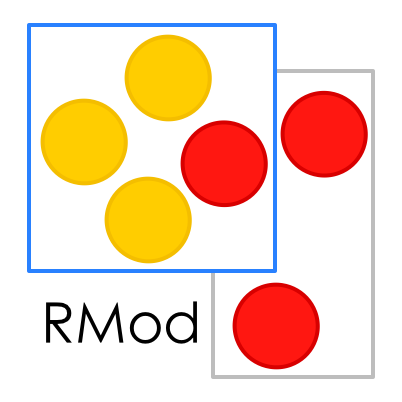
\includegraphics[width=0.3\textwidth]{/home/cyber/Work/Pharo/Booklet-Polyglot/_result/pdf/Chapters/Chapter2/figures/rmod.png}\caption{\label{/home/cyber/Work/Pharo/Booklet-Polyglot/_result/pdf/Chapters/Chapter2/figures/rmod.png}}\end{center}
\end{figure}





\bibliographystyle{alpha}
\bibliography{book.bib}

% lulu requires an empty page at the end. That's why I'm using
% \backmatter here.
\backmatter

% Index would go here

\end{document}
